
\section{Experiments}
\label{sec:expts}

We perform three different feature selection methods on our data. The first, which we call the "basic" feature selection is simply having each of the 784 pixel color values as an individual feature for the model. Secondly, we apply a Canny edge detection which is a multi-stage edge detector. First a Gaussian filter is applied to reduce noise in the image, and lastly edges are thinned down to a length of one pixel. The sigma parameter in the Canny filter determines the edge intensity. The Sklearn documentation provides an example image for what each step looks like. This can be seen in figure 3, where the first image has been through the Gaussian filter, and the other two images have been run through the Canny filter with differing sigma parameters. Like the basic feature selection, each of the 784 pixel values in the new image are an individual feature.

\begin{figure}[!h]
    \centering
    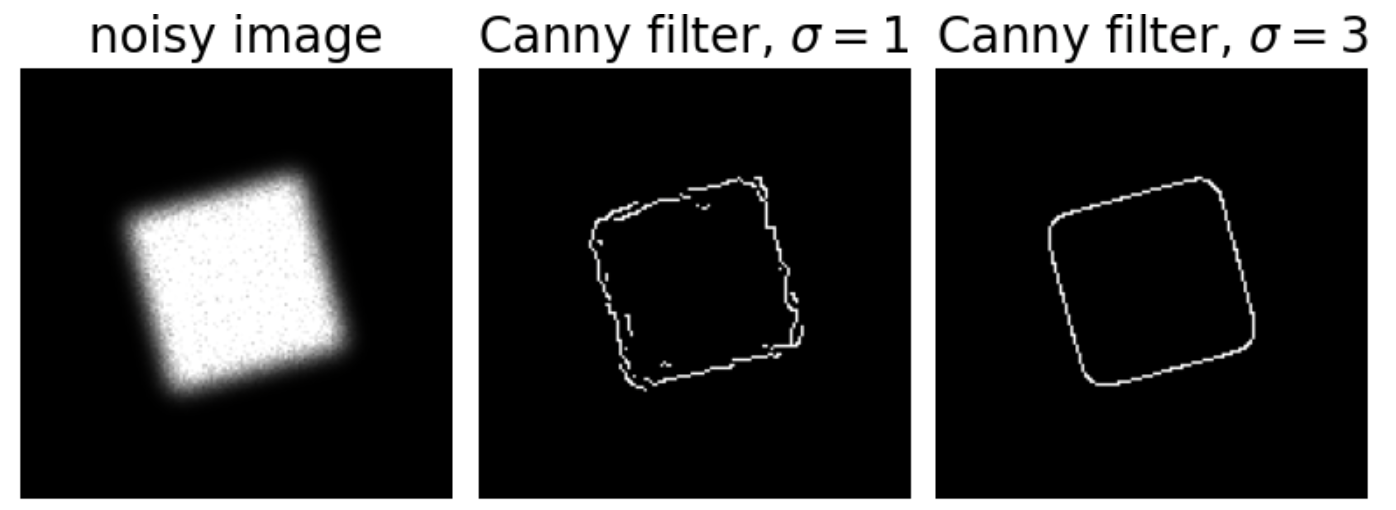
\includegraphics[width=3.33in]{canny_sklearn.png}
    \caption{Sklearn Example of Canny Filter (Source: Sklearn documentation)}
    \label{fig:my_label}
\end{figure}

In Figure 4, you can see the results of the edge detection applied to the original image with a sigma value of 1. This allows for an accurate edge detection to capture the shape of the clothing without confusing contrast in patterns/colors for edges. We expect that edge detection will reduce the noise created by different colors and patterns on the clothing and make the classification more accurate by only focusing on the general shape of each garment.

\begin{figure}[!h]
    \centering
    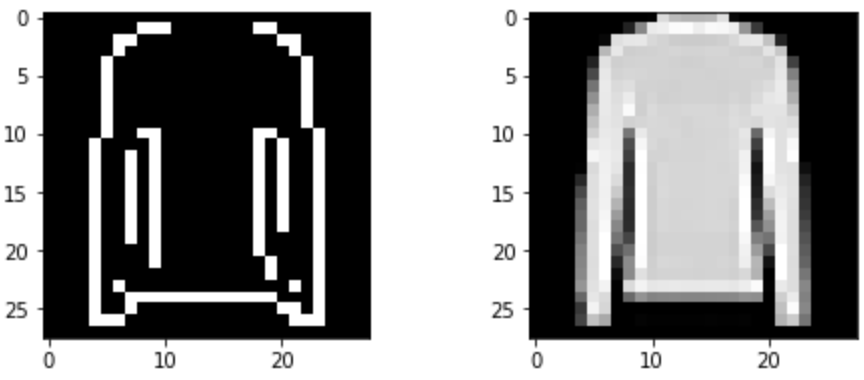
\includegraphics[width=3.33in]{canny_ex.png}
    \caption{Edge Detection (Left), Original Image (Right)}
    \label{fig:my_label}
\end{figure}

The last feature selection is a combination of the two that we are calling the "combined" feature selection. Instead of the 784 features that the basic and Canny models have, the combined model has 1568 features (784 without a filter, 784 with the filter).

Next, we run these three different sets of features through two different classification models. We use a K-nearest neighbors model (KNN) and a logistic regression model. Lastly, we created a baseline model that would always select the most common article of clothing. This provides us with a metric besides the Zhou and Bossard results to test our performance against.

Like the Zhou and Bossard paper, we used an F1 score as the measure of accuracy, as it takes into account both precision and recall by counting false negatives and false positives. Specifically we used an F1 Macro score which takes the arithmetic mean of the F1 scores for each class.

KNN classifies an input by finding the k-nearest neighbors of that given input (we use euclidean distance) and classifying that input by choosing the most common class between those k neighbors.

For the KNN model, we first tuned the value of k by using cross-validation on a smaller subset of the testing dataset (1000 images) to estimate the best value for k. We found that for the basic feature selection model, a value of $k=8$ was the most accurate on the random 1000 images. Alternatively, for the Canny and combined feature selection methods, we found that a smaller value of $k=5$ was the most accurate, as can be seen in figures 5, 6, and 7.

\begin{figure}[!h]
    \centering
    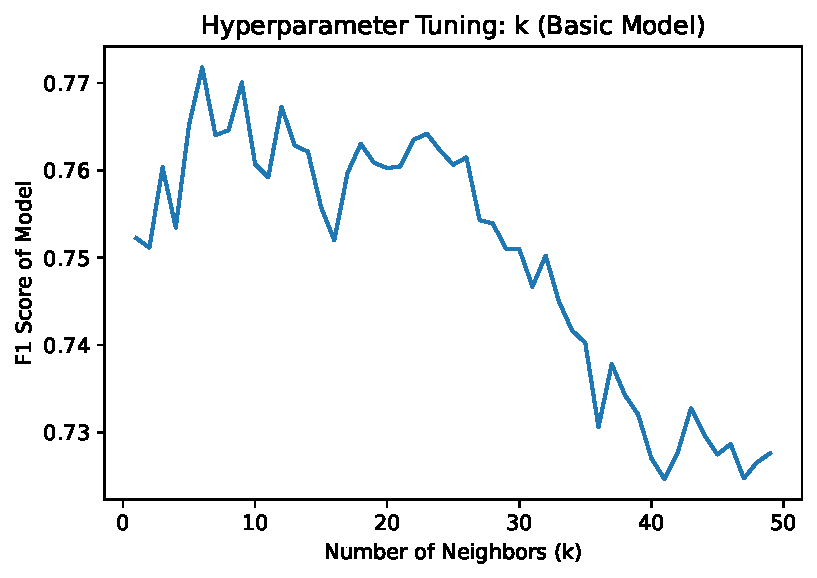
\includegraphics[width=3.3in]{tuning_k_basic.pdf}
    \caption{Basic Feature Selection Model: Tuning k}
    \label{fig:my_label}
\end{figure}

\begin{figure}[!h]
    \centering
    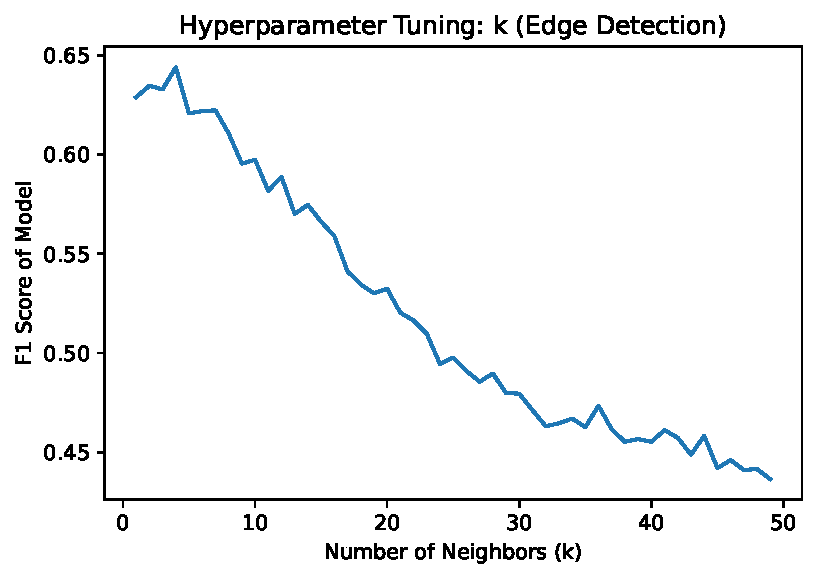
\includegraphics[width=3.3in]{tuning_k_canny.pdf}
    \caption{Canny Feature Selection Model: Tuning k}
    \label{fig:my_label}
\end{figure}

\begin{figure}[!h]
    \centering
    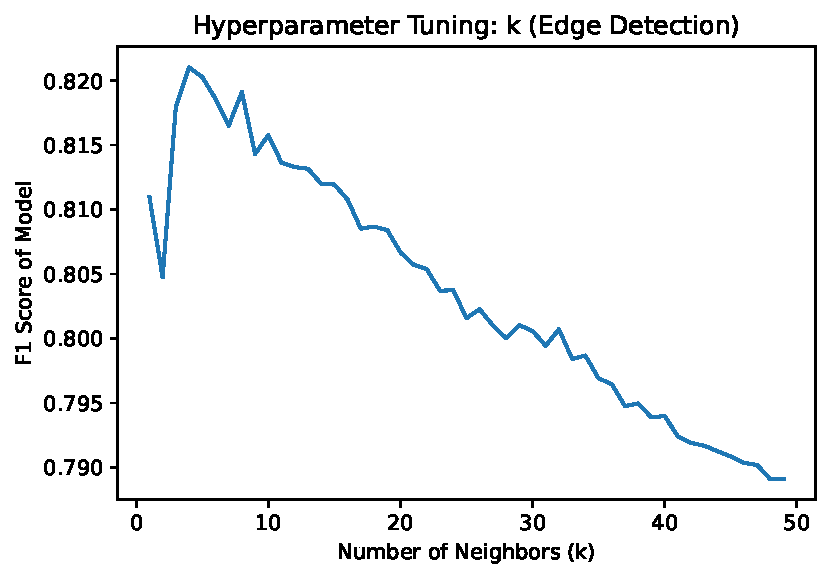
\includegraphics[width=3.3in]{tuning_k_combine.pdf}
    \caption{Combined Feature Selection Model: Tuning k}
    \label{fig:my_label}
\end{figure}

For the logistic regression, we use the "newton-cg" solver built into the sklearn library which has a more complex cost function used to enable a multi-class classification rather than the simple binary classification choice possible with the basic form of the logistic regression.

Additionally, for every model, we used cross-validation to get an idea of how accurate our models are without contaminating our testing data. It prevents us from completely over-fitting the testing data as the the intermediate accuracy measure can give an idea of how the model handles unseen data.

We expect that, for both feature selection models, either KNN or logistic regression will outperform the other for the basic, Canny, and combined feature selection methods. KNN is non-parametric and can therefore capture more complexities, and thus is more likely to overfit if the true behavior is not too complex (i.e. linear or polynomial). On the other hand, logistic regression is more likely to predict less complex behavior and therefore underfit a complex model. We assume that KNN will be better suited for a computer vision problem because each image contains many features and clothing classification is a complex problem.